\documentclass[14pt]{extarticle}

\usepackage{fontspec}
\setmainfont{Times New Roman}

% размер полей
\usepackage{geometry}
\geometry{a4paper, top=2cm, bottom=2cm, right=1.5cm, left=3cm}

 %debugging
%\usepackage{showframe}

% полуторный интервал
\usepackage{setspace}
\onehalfspacing

% абзацный отступ
\setlength{\parindent}{1.25cm}

% выравнивание текста по ширине
\sloppy

% списки
\usepackage{calc} % арифметические операции с величинами
\usepackage{enumitem}
\setlist{
    nosep,
    leftmargin=0pt,
    itemindent=\parindent + \labelwidth - \labelsep,
}

% подписи к рисункам и таблицам
\usepackage{caption}
\renewcommand{\figurename}{Рисунок}
\renewcommand{\tablename}{Таблица}
\DeclareCaptionFormat{custom}
{
    \textit{#1#2#3}
}
\DeclareCaptionLabelSeparator{custom}{. }
\captionsetup{
    % хз какой это размер - 12 или нет, но выглядит меньше 14
    font=small,
    format=custom,
    labelsep=custom,
}

% картинки
\usepackage{graphicx}

% колонтитулы
\usepackage{fancyhdr}

% картинки и таблицы находятся именно в том месте текста где помещены (атрибут H)
\usepackage{float}

% таблицы
\usepackage{tabularray}

\graphicspath{ {2.2/models/} }
\usepackage{hyperref}
\usepackage{upgreek}
\begin{document}
\pagestyle{fancy}
\fancyhead{}
% disable header
\renewcommand{\headrulewidth}{0pt}
\singlespacing

\newpage
\begin{center}
    Министерство науки и высшего образования Российской Федерации
    Федеральное государственное автономное образовательное учреждение

    высшего образования

    \guillemotleft МОСКОВСКИЙ ПОЛИТЕХНИЧЕСКИЙ УНИВЕРСИТЕТ\guillemotright

    (МОСКОВСКИЙ ПОЛИТЕХ)
\end{center}
\noindent
\bigbreak
\bigbreak
\bigbreak
\bigbreak
\begin{center}
    \textbf{ОСНОВНЫЕ ПОНЯТИЯ, ТЕРМИНЫ И РАСПРЕДЕЛЕНИЯ ИЗ
ТЕОРИИ ВЕРОЯТНОСТЕЙ}
    \bigskip
    \bigskip
    \bigskip
    \bigskip
    \bigskip

    Лабораторная работа 2.2

    По курсу \guillemotleft Надёжность информационных систем\guillemotright
    \bigskip

    \bigbreak
    \bigbreak
    \bigbreak
    \bigbreak
\end{center}
\noindent
\bigbreak
\bigbreak
\bigbreak
\bigbreak
\bigbreak
\bigbreak
\bigbreak
\bigbreak
\bigbreak
\bigbreak
\hfill Выполнил

\hfill Дубровских Н.Е.

\hfill Группа 221-361
\bigbreak
\bigbreak
\bigbreak
\hfill Проверил

\hfill Маковей С.О.
\vfill
\begin{center}
    Москва, 2024
\end{center}
\newpage
\onehalfspacing


\begin{center}
    \textbf{Лабораторная работа 2.2}

    \textbf{Основные распределения, используемые в
теории надежности. Распределение Бернулли. Геометрическое
распределение. Экспоненциальное распределение.
Гиперэкспоненциальное распределение. Биномиальное распределение.}
\end{center}

К \textbf{основным целям} лабораторной работы следует отнести:

\begin{itemize}
    \item формирование у студентов понимания важности развития и применения средств теории вероятностей в современных информационных системах и технологиях;
    \item ознакомление студентов с основными распределениями теории вероятностей.
\end{itemize}

К \textbf{основным задачам} лабораторной работы следует отнести:

\begin{itemize}
    \item анализа состояния и тенденций развития теории вероятностей;
    \item развитие навыков изучения истории и областей применения методов теории вероятностей;
    \item развитие навыков классификации средств генераторов последовательностей случайных чисел.
\end{itemize}
\bigskip

\pagebreak

\begin{center}
\textbf{ОТЧЁТ ПО ВЫПОЛНЕНИЮ}
\end{center}

\textbf{Задача № 1}

ИИ выявил 5000 доброкачественных изделий. Вероятность того, что
отобранное изделие является бракованным, равна 0,0002. Найти
вероятность того, что среди всех изделий: а) три негодных изделия; б) не
более трёх повреждённых изделия.

\textbf{Решение}

\textbf{a)}

Определим интенсивность события

$\lambda = n \cdot p = 5000 \cdot 0.0002 = 1$

Применим закон распределения Пуассона

$P_n(k) = \frac{\lambda^k}{k!}e^{-\lambda}$

$P_{5000}(3) = \frac{1^3}{3!}e^{-1} = \frac{1}{6}e^{-1} = \frac{1}{6e} = 0.061313240195240384 \approx 0.06$

\textbf{б)}

$P = P_{5000}(0) + P_{5000}(1) + P_{5000}(2) + P_{5000}(3) = \frac{1^0}{0!}e^{-1} + \frac{1^1}{1!}e^{-1} + \frac{1^2}{2!}e^{-1} + \frac{1^3}{3!}e^{-1} = \frac{1}{e} + \frac{1}{e} + \frac{1}{2e} + \frac{1}{6e} = \frac{2}{e} + \frac{1}{2e} + \frac{1}{6e} = \frac{12}{6e} + \frac{3}{6e} + \frac{1}{6e} = \frac{16}{6e} = \frac{8}{3e} = 0.9810118431238462 \approx 0.98$

\textbf{Задача 2.}

Случайная величина X имеет геометрическое распределение с
параметром p=0,2. Построить ряд распределения случайной величины X.
Построить многоугольник распределения. Определить математическое
ожидание, дисперсию, среднее квадратическое отклонение величины X.

\textbf{Решение}

$P(X = k) = (1 - p)^k \cdot p = (1 - 0.2)^k \cdot 0.2 = 0.8^k \cdot 0.2$

Ряд распределения

\begin{table}[H]
    \centering
\begin{tabular}{|c|c|c|c|c|c|c|c|}
    \hline
    X & 0 & 1 & 2 & 3 & ... & k & ...\\
    \hline
    P & 0.2 & 0.16 & 0.128 & 0.1024 & ... & $0.8^k \cdot 0.2$ & ...\\
    \hline
\end{tabular}
\end{table}

Многоугольник распределения

\noindent
\begin{minipage}[H]{\linewidth}
    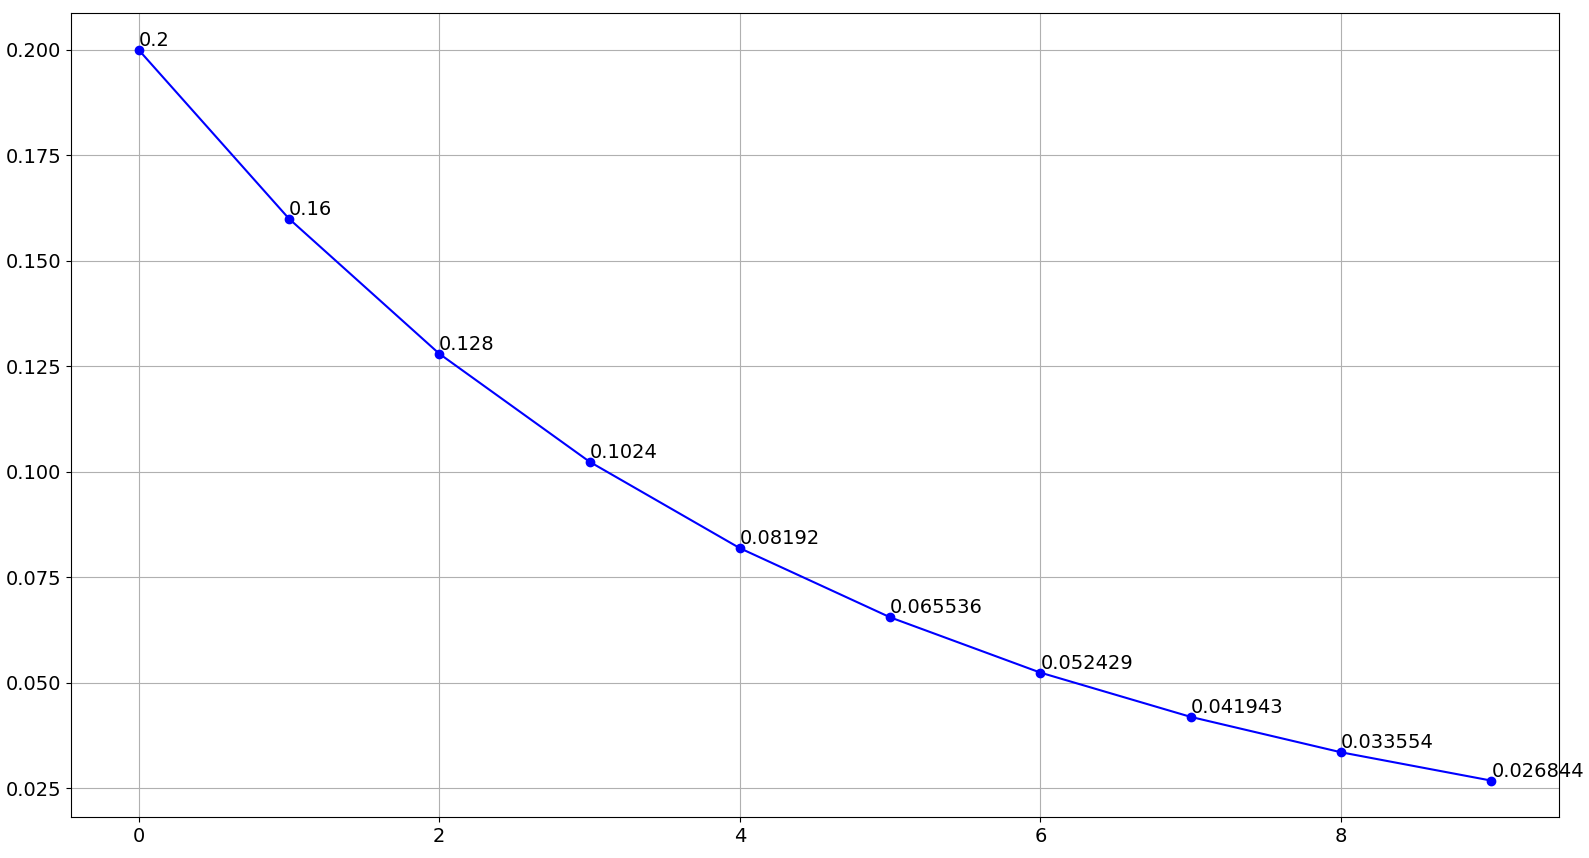
\includegraphics[width=\linewidth]{f}
\end{minipage}
\bigskip

Определим математическое ожидание

$M(X) = \frac{q}{p} = \frac{0.8}{0.2} = 4$

Определим дисперсию

$D(X) = \frac{q}{p^2} = \frac{0.8}{0.2^2} = 20$

Определим среднее квадратическое отклонение

$\sigma(X) = \sqrt{D(X)} = \sqrt{20} \approx 4.472$

\bigskip

\textbf{Задача 3.}

Математическое ожидание случайной величины, распределенной
по показательному закону:

$M(X) = \frac{1}{\lambda}$

Дисперсия случайной величины, распределенной по
показательному закону:

$D(X) = \frac{1}{\lambda^2}$

Среднее квадратическое отклонение случайной величины,
распределенной по показательному закону:

$\sigma(X) = \frac{1}{\lambda}$

Коэффициенты асимметрии и эксцесса для показательного
распределения:

$A_S = 2; E_S = 6$

Таким образом, математическое ожидание и среднее
квадратическое отклонение экспоненциального распределения равны
между собой.

Случайная величина $\xi$ задана функцией распределения

$F_\xi(x) =
\begin{cases} 
1 - e^{-4x}, & \text{при } x > 0, \\
0, & \text{при } x \leq 0.
\end{cases}$

Определить математическое ожидание и среднее квадратическое
отклонение этого распределения.

Найти вероятность того, что случайная величина примет значение
от 0,2 до 1.

\textbf{Решение}

$\lambda = 4$

Определим математическое ожидание и среднее квадратическое отклонение

$M(\xi) = \sigma(\xi) = \frac{1}{\lambda} = \frac{1}{4} = 0.25$

Определим вероятность того, что случайная величина примет значение
от 0,2 до 1

$P(0.2 < \xi < 1) = F_{\xi}(1) - F_{\xi}(0.2) = 1 - e^{-4 \cdot 1} - (1 - e^{-4 \cdot 0.2}) = 1 - e^{-4} - 1 + e^{-0.8} = e^{-0.8} - e^{-4} = 0.4310133252284874 \approx 0.431$

\end{document}
